 \begin{figure}[h!]
  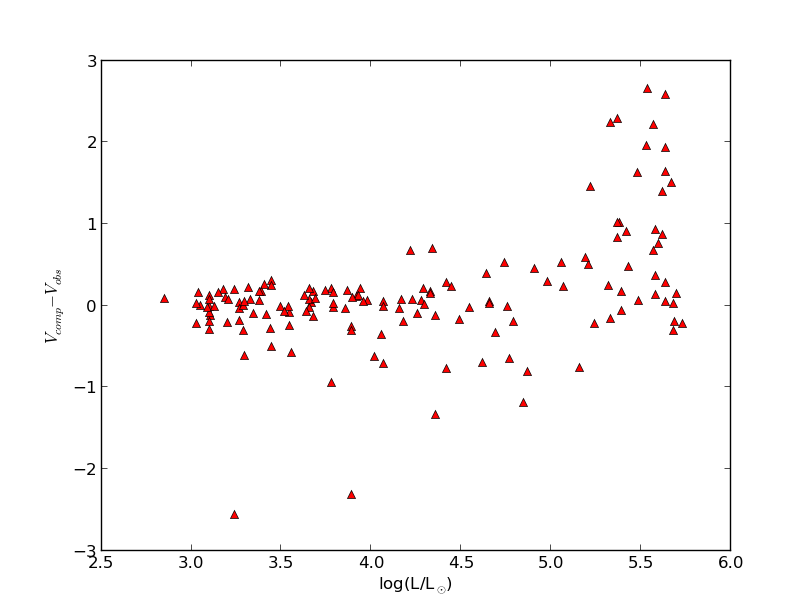
\includegraphics[width=0.9\textwidth]{diffmaglogL}
  \caption{Difference between computed and observed magnitudes as a function of $\log(L/L_\odot)$}
 \end{figure}
 
 The theoretical magnitudes ($V_{comp}$) were computed using stellar radius, luminosity and distance. The observational magnitudes ($V_{obs}$)
 were taken from a sample of 150 stars between M=5M$_\odot$ and M=48M$_\odot$ from \citep{2014A&A...570L..13C}
 
 Figure \ref{diffmagmass} shows the difference between computed and observed magnitudes as a function of mass. There is a significant
 deviation towards higher $V_{comp}$ at high masses. This can be explained using Figure \ref{castroetal}:
 \begin{figure}
  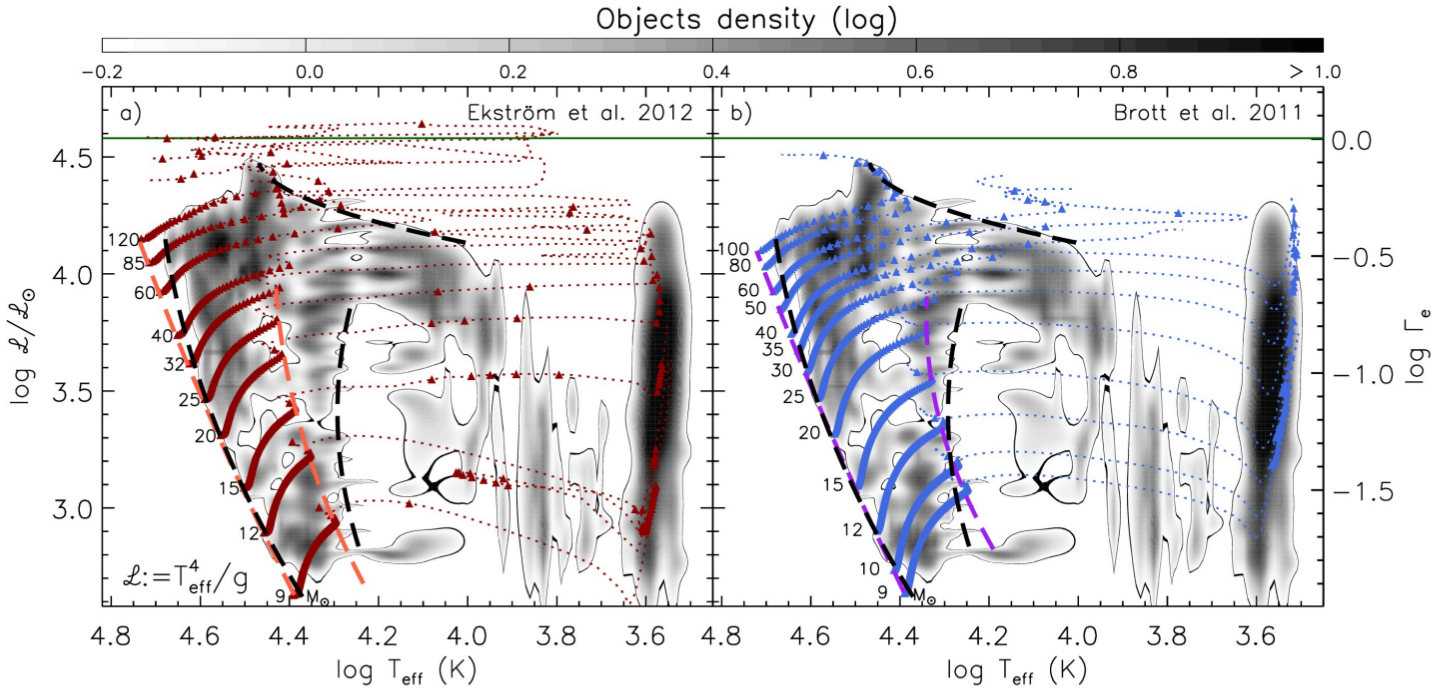
\includegraphics[width=\textwidth]{Castroetal}
  \caption{Grey scale representation of the probability density distribution of the location of 575 Galactic stars in the sHRD.
  Overlayed are stellar evolution tracks for non-rotating stars with solar composition a)\citet{2012A&A...537A.146E}
  and b)\citet{2011yCat..35309115B}. The ZAMS and TAMS positions of the models are connected through orange and purple dashed lines.
  Red and blue triangles are placed on the tracks separated by 0.1 Myr \citep{2014A&A...570L..13C}\label{castroetal}}
 \end{figure}

 My code uses an evolutionary model similar to model a). $V_{obs}$ however is obtained using a model similar to model b).
 Model b) accounts for convective overshooting to a higher degree and thus the lifetime of stars is expanded. This would account for
 minor deviations. Because of the difference in position of TAMS in the HRD, \textbf{I STILL DON'T GET IT}.
 The massive deviations between $M=25M_\odot$ and $M\approx 43M_\odot$ can be explained by taking into account inflation. 
 Near TAMS on the main sequence massive stars will undergo an expansion of their envelopes. This gives rise to a big shift on the
 HRD.
 

 
 \begin{figure}[h!]
  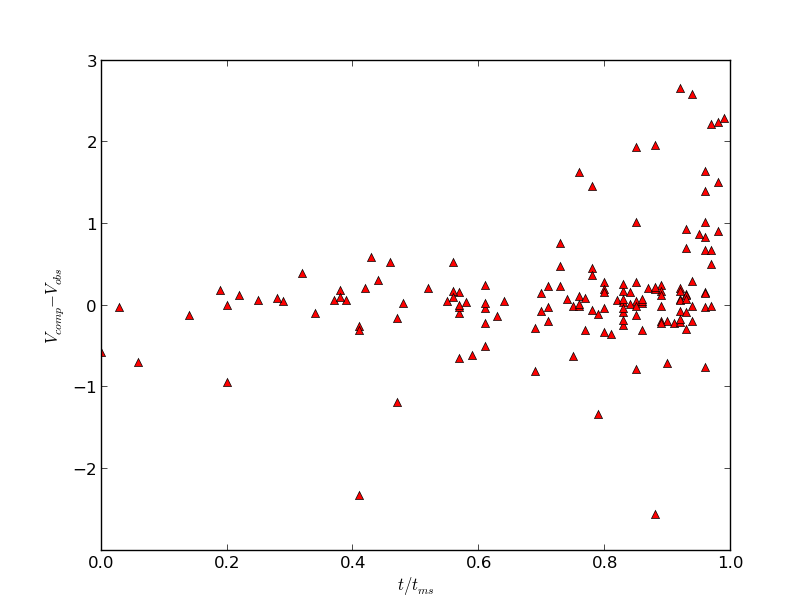
\includegraphics[width=0.9\textwidth]{diffmagfracms}
  \caption{Difference between computed and observed magnitudes as a function of age}
 \end{figure}
 
 
 
 The deviation to negative values is mostly caused by extinction. It is most prevalent in lower absolute ages. 
 Stars of lower ages are primarily found in regions of active star formation. This would mean, that they are found in regions
 of high gas density. This gas will cause extinction and thus increase $V_{obs}$. My model for extinction does not take into account 
 these density fluctuations.
 